\documentclass[final]{beamer}

% ====================
% Packages
% ====================



\usepackage[orientation=portrait,size=a0,scale=1.0]{beamerposter}
\usetheme{gemini}
\usecolortheme{ENSA}
\usepackage{graphicx}
\usepackage{booktabs}
\usepackage{amsmath,amssymb,bm}
\usepackage{tikz}
\graphicspath{{../results/figures/}}

% ====================
% Lengths
% ====================

% (N+1)*sepwidth + N*colwidth = paperwidth
\newlength{\sepwidth}
\newlength{\colwidth}
\setlength{\sepwidth}{0.025\paperwidth}
\setlength{\colwidth}{0.3\paperwidth}
\newcommand{\separatorcolumn}{\begin{column}{\sepwidth}\end{column}}

\newcommand{\dto}{\Delta t_{\mathrm{obs}}}
\newcommand{\tc}{t_{\mathrm{char}}}
\newcommand{\lmax}{\lambda_{\max}}

% ====================
% Title
% ====================

\title{Learning and Discovering Chaotic Dynamics from Sparse, Noisy Observations}
\author{Paul Christopher Aim\'e}
\institute[ENSA Marrakech]{\'Ecole Nationale des Sciences Appliqu\'ees de Marrakech, Universit\'e Cadi Ayyad}

% ====================
% Body
% ====================

\begin{document}

\begin{frame}[t]
\begin{columns}[t]
\separatorcolumn
\begin{column}{0.95\paperwidth}
  \begin{alertblock}{Reconstructed attractors at coarse sampling: free runs of the identified models}
    \centering
    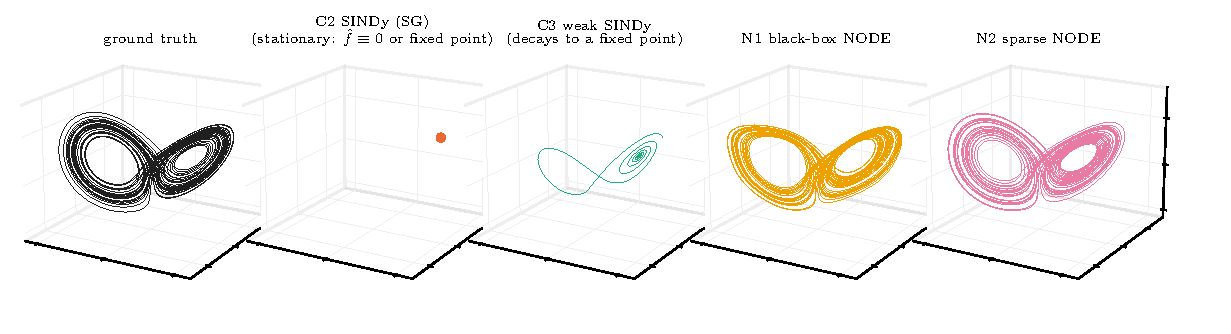
\includegraphics[width=0.88\linewidth,trim=0 26 0 4,clip]{fig06_gallery_lorenz_dt0.267_n0.01.pdf}
    \vspace{0.3ex}

    \raggedright
    Lorenz-63 sampled every $\dto=0.2$ (about 4 samples per oscillation), $\varepsilon=1\%$. Free runs over $60\,\tc$. SINDy (SG) selects $\hat f\equiv0$, and weak SINDy decays to a fixed point. The black-box NODE stays near the attractor but its equations are wrong. The sparse NODE recovers
\[
\dot x=-9.59x+9.73y,\quad \dot y=28.03x-1.02y-1.00xz,\quad \dot z=-2.66z+1.00xy
\]
(plus two terms of size $\sim\!0.02$). Median coefficient error over seeds: \textbf{0.05}, against $\ge 2.4$ for every classical method.
  \end{alertblock}
\end{column}
\separatorcolumn
\end{columns}

\begin{columns}[t]
\separatorcolumn

%%%%%%%%%%%%%%%%%%%%%%%%%%%%%%%%%%%%%%%%%%%%%%%%%%%%%%%%%%%%%%%%%% COLUMN 1
\begin{column}{\colwidth}

  \begin{block}{Question}
    Given a few short, noisy, coarsely sampled records of a chaotic system $\dot x=f(x)$, can we
    \textbf{recover the equations}, \textbf{forecast} up to the predictability limit, and
    \textbf{know when not to trust} the model? And when do neural ODEs beat sparse regression?
  \end{block}

  \begin{block}{Problem formulation}
    \heading{Observations}
    \[
      y^{(e)}_k = x^{(e)}(t_k) + \eta^{(e)}_k,\qquad \eta\sim\mathcal N\big(0,\varepsilon^2\Sigma_x\big),
    \]
    on a grid of step $\dto$, for $E=4$ short experiments.
    \heading{Sparse library model}
    \[
      f(x)=\bm\Xi^\top\theta(x),\quad \theta(x)=\big(1,\,x_i,\,x_ix_j\big)_{i\le j},\quad \bm\Xi\ \text{sparse}.
    \]
    Coordinates are scaled without centring, $z=S^{-1}x$, $\tau=t/\tc$, so that $\tilde{\bm\Xi}=\tc\,C\bm\Xi S^{-1}$ keeps the support.
    \heading{Why trajectory matching is hard on chaos}
    The sensitivity $U=\partial x/\partial\vartheta$ obeys $\dot U=J(x)U+\partial_\vartheta f$, so $\|U(t)\|\sim e^{\lmax t}$.
    The single-shooting loss $\mathcal L_T$ gets rough, and its convex-like basin shrinks like $e^{-\lmax T}$.
    \heading{Multiple shooting with latent states}
    \begin{align*}
      \mathcal J_K(\vartheta,S)=&\ \tfrac{1}{|\mathcal W|K}\textstyle\sum_{i,k}\big\|\Phi^{t_{i+k}-t_i}_\vartheta(S_i)-y_{i+k}\big\|^2_{\Sigma^{-1}}\\
      &+\tfrac{w}{N}\textstyle\sum_i\|S_i-y_i\|^2_{\Sigma^{-1}}
    \end{align*}
    Sensitivities are bounded by $e^{\lmax K\dto}$, independently of the record length.
  \end{block}

  \begin{block}{Systems and protocol}
    \begin{columns}[T]
      \begin{column}{0.48\colwidth}
        \centering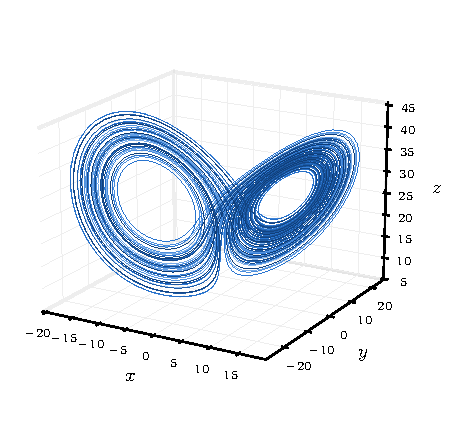
\includegraphics[width=\linewidth]{fig01_attractor_lorenz.pdf}\\
        Lorenz-63, $\lmax\tc=0.68$
      \end{column}
      \begin{column}{0.48\colwidth}
        \centering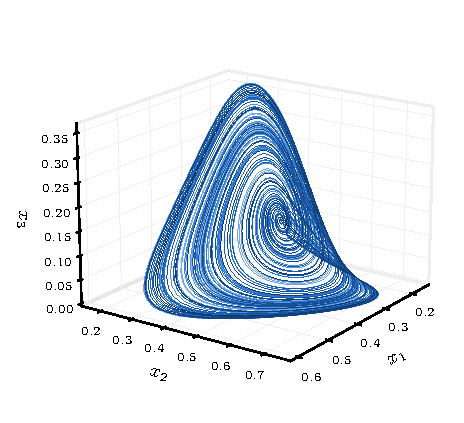
\includegraphics[width=\linewidth]{fig01_attractor_lv4.pdf}\\
        competitive LV ($d=4$), $\lmax\tc=0.67$
      \end{column}
    \end{columns}
    \vspace{1ex}
    \begin{itemize}
      \item 4 experiments, total $\tfrac{80}{3}\tc$; $\dto/\tc\in\{\tfrac1{75},\tfrac1{15},\tfrac2{15},\tfrac4{15}\}$; $\varepsilon\in\{0,\dots,20\}\%$; 3 seeds.
      \item \textbf{C1} OLS \;\textbf{C2} SINDy (FD / Savitzky--Golay) \;\textbf{C3} weak SINDy
      \item \textbf{N1} black-box NODE + symbolic distillation \;\textbf{N2} sparse-library NODE
      \item All hyper-parameters are selected on held-out blocks; no estimator sees the true $\bm\Xi$.
    \end{itemize}
  \end{block}

  \begin{block}{N2: sparse-library neural ODE}
    \begin{enumerate}
      \item Levenberg--Marquardt on the one-step flow map, $\Phi^{\dto}_{\Xi}(y_i)\approx y_{i+1}$.
      \item L-BFGS on $\mathcal J_K$ over $(\Xi,S)$ with continuation $K=1,2,3,5,8,\dots$
      \item Multistart over $\{0,\ \Xi_{\rm OLS}\}$ (N2-WS: $+\,\Xi_{\rm WSINDy}$).
      \item Sequential thresholding with trajectory-matching refits along a $\lambda$-path.
    \end{enumerate}
  \end{block}

\end{column}

\separatorcolumn

%%%%%%%%%%%%%%%%%%%%%%%%%%%%%%%%%%%%%%%%%%%%%%%%%%%%%%%%%%%%%%%%%% COLUMN 2
\begin{column}{\colwidth}



  \begin{block}{Benchmark: equation recovery}
    \centering
    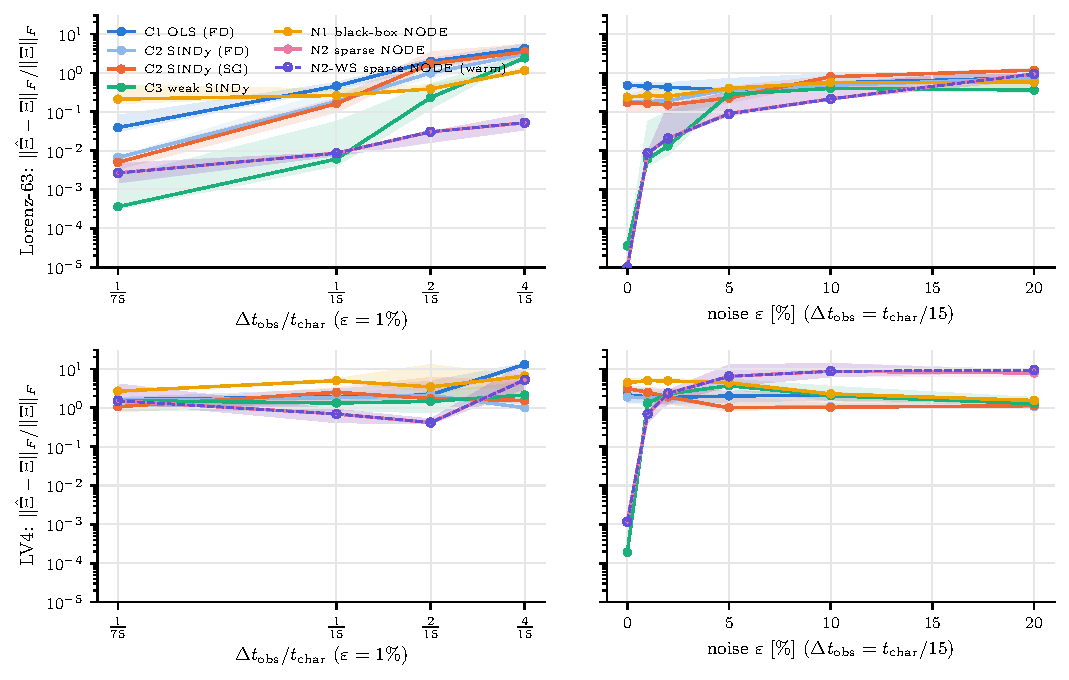
\includegraphics[width=\linewidth]{fig06_benchmark_coef.pdf}
    \vspace{0.5ex}

    \raggedright
    Median relative coefficient error $\|\hat\Xi-\Xi\|_F/\|\Xi\|_F$ over 3 seeds. Left: sampling sweep at $\varepsilon=1\%$. Right: noise sweep at $\dto=\tc/15$.
\begin{itemize}
  \item \textbf{Lorenz:} weak SINDy is best at dense sampling ($4\cdot10^{-4}$). The sparse NODE wins once $\dto\ge 2\tc/15$: $0.031$ against $0.23$, and $0.052$ against $2.4$.
  \item \textbf{LV4:} recovery only from noise-free data. The library's condition number on the attractor is $\approx3\cdot10^4$, so 1\% noise is already too much for \emph{every} estimator.
  \item The distilled black-box equations are dense: error $0.21$--$1.15$ on Lorenz.
\end{itemize}
  \end{block}

  \begin{block}{Forecasting: in- and out-of-distribution}
    \centering
    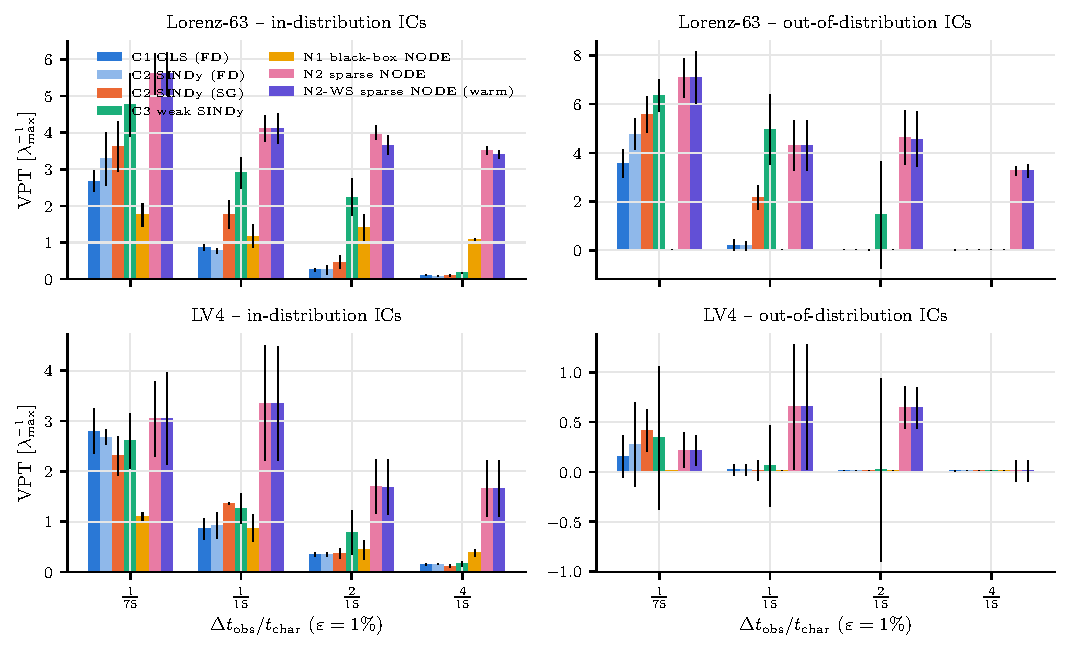
\includegraphics[width=\linewidth]{fig06_vpt.pdf}
    \vspace{0.5ex}

    \raggedright
    Valid prediction time (normalised error $<0.4$) in Lyapunov times, at $\varepsilon=1\%$. The exact field reaches $11.3$ (Lorenz) and $8.1$ (LV4) with the same RK4 integrator.
\begin{itemize}
  \item The sparse NODE has the longest in-distribution VPT at every $\dto$, on both systems: $3.5$ at $\dto=0.2$ on Lorenz, against $\le0.17$ for the classical methods.
  \item \textbf{Out of distribution} (initial conditions $\ge2\sigma$ from the attractor) the black-box NODE fails at once (VPT $0.015$). Correct sparse models extrapolate (Lorenz N2: $3.3$--$7.1$).
\end{itemize}
  \end{block}

\end{column}

\separatorcolumn

%%%%%%%%%%%%%%%%%%%%%%%%%%%%%%%%%%%%%%%%%%%%%%%%%%%%%%%%%%%%%%%%%% COLUMN 3
\begin{column}{\colwidth}

  \begin{block}{Loss landscapes and nonconvex optimisation}
    \centering
    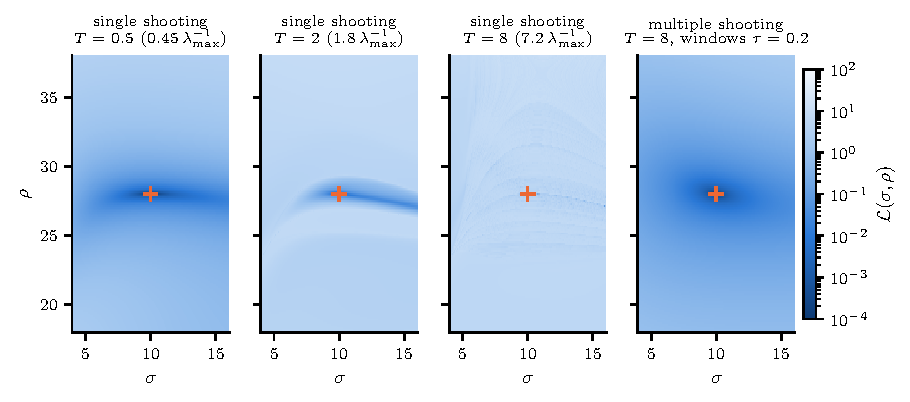
\includegraphics[width=\linewidth]{fig04_landscape_sigma_rho.pdf}
    \vspace{0.5ex}

    \raggedright
    \begin{itemize}
  \item Exact $\mathcal L(\sigma,\rho)$: single shooting becomes a flat surface with a needle-like minimum as $T$ grows. Multiple shooting stays smooth.
  \item The median $\|\nabla\mathcal L_T\|$ grows like $e^{0.68T}$ ($\lmax=0.91$).
  \item 96 random restarts for $(\sigma,\rho,\beta)$: single shooting with $T=4$ succeeds 0\% of the time, and multiple shooting with windows of $0.2$ \textbf{100\%}.
  \item Full library from random starts: continuation succeeds for 100\% of them at $\dto=0.05$ and for up to 100\% at $\dto=0.2$; direct training at the longest window succeeds for \textbf{0\%}.
\end{itemize}
  \end{block}

  \begin{block}{Uncertainty quantification}
    \centering
    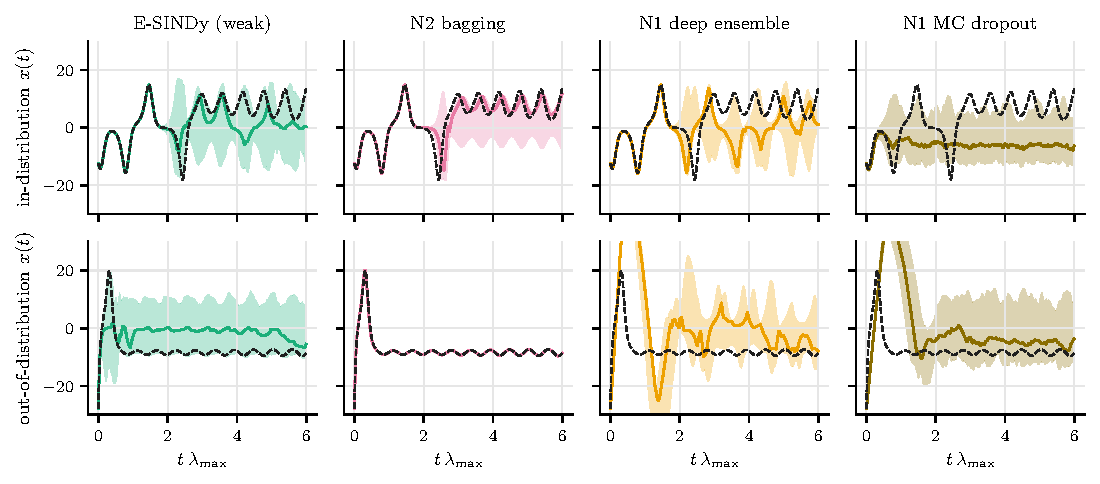
\includegraphics[width=\linewidth]{fig05_uq_bands.pdf}
    \vspace{0.5ex}

    \raggedright
    Ensemble forecasts, Lorenz with $\dto=0.05$ and $\varepsilon=1\%$. Top: in distribution. Bottom: out of distribution.
\begin{center}\small
\begin{tabular}{lccc}
\toprule
 & coverage (90\%) & CRPS & OOD/ID spread \\
 & ID / OOD & ID / OOD & \\
\midrule
E-SINDy (weak) & \textbf{0.87} / \textbf{0.93} & 0.16 / 0.22 & 15.4 \\
N2 bagging & 0.18 / 0.11 & \textbf{0.10} / \textbf{0.07} & 3.9 \\
N1 deep ensemble & 0.41 / 0.47 & 0.51 / 1.35 & 11.9 \\
N1 MC dropout & 0.67 / 0.64 & 0.64 / 0.96 & 1.1 \\
\bottomrule
\end{tabular}
\end{center}
The bootstrap of the weak regression is calibrated, and window bagging is accurate but over-confident. Deep ensembles flag distribution shift; trajectory-wise MC dropout does not.
  \end{block}

  \begin{alertblock}{Take-aways}
    \begin{enumerate}
  \item The gain of neural ODEs for discovery comes from \textbf{matching trajectories}, not from neural networks. The sparse-library NODE extends recovery to $\sim\!4$ samples per period.
  \item On chaotic flows that gain depends on \textbf{multiple shooting, continuation and multistart}. Single shooting fails beyond about one Lyapunov time.
  \item Black-box NODEs give \textbf{no equations and no extrapolation}.
  \item Identifiability is a property of the \textbf{data}: check $\sigma_{\min}(\Theta)$ before trusting any estimator.
\end{enumerate}
  \end{alertblock}

  \begin{block}{References}
    \footnotesize
    Brunton, Proctor \& Kutz, \emph{PNAS} 2016 \textbullet{}
    Messenger \& Bortz, \emph{MMS} 2021 \textbullet{}
    Fasel et al., \emph{Proc.\ R.\ Soc.\ A} 2022 \textbullet{}
    Chen et al., \emph{NeurIPS} 2018 \textbullet{}
    Bock \& Plitt, \emph{IFAC} 1984 \textbullet{}
    Ribeiro et al., \emph{Automatica} 2020 \textbullet{}
    Vano et al., \emph{Nonlinearity} 2006 \textbullet{}
    Lakshminarayanan et al., \emph{NeurIPS} 2017 \textbullet{}
    Gal \& Ghahramani, \emph{ICML} 2016 \textbullet{}
    Li et al., \emph{NeurIPS} 2018
  \end{block}

\end{column}

\separatorcolumn
\end{columns}
\end{frame}

\end{document}
